\newpage
\section{Лекция 15}
\subsection{Теоремы Перрона}
\begin{theorem}[О сжимающем отображении]
    Существует единственное $\bar x\geqslant 0:~\varphi(\bar x)=\bar x$ --- неподвижная точка, то есть $$\cfrac{1}{|Ax|_1}A\bar x=\bar x$$
$$Ax=\hat \lambda x,~~\hat \lambda=|Ax|_1$$
\end{theorem}
\begin{theorem}[Перрона]
    Если $A>0$ (то есть все $a_{ij}>0$), то у матрицы $A$ существует положительное собственное значение $\hat \lambda =\hat \lambda_A:~~\hat \lambda =\rho(A)$ и $\hat \lambda>|\lambda|$ для всех остальных собственных значений $\lambda$ матрицы $A$. Этому собственному значению отвечает положительный собственный вектор $\hat x>0$ --- единственный с точностью до пропорциональности: в частности $\hat \lambda$ --- простое, то есть кратности один.
\end{theorem}
\begin{proof}
    Рассмотрим отображение $\bar x \mapsto A \bar x \to \cfrac{A\bar x}{|Ax|_1}$.\\
\begin{center}
    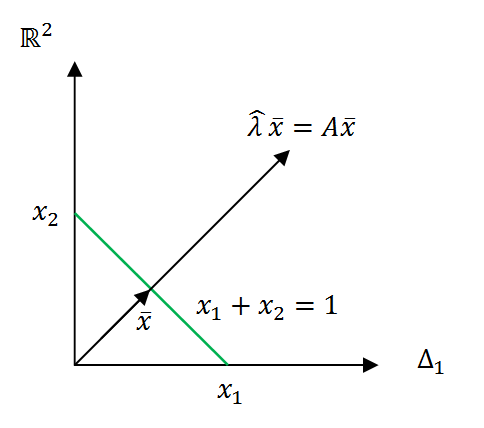
\includegraphics[scale=0.8]{l15_1.png}
    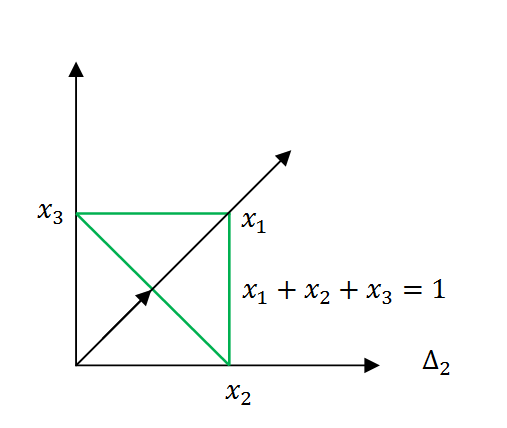
\includegraphics[scale=0.8]{l15_2.png}\\
\end{center}
Рассмотрим на множестве $\Delta=\Delta_{n-1}=\{ x_1\geqslant \bar 0, \cdots, x_n\geqslant \bar 0 ~~|~~ x_1+\cdots +x_n=1 \}$.\\
При отображении $A:~\mathbb{R}^n\to \mathbb{R}^n$ множество $\mathbb{R}^n_{\geqslant 0}$, где $x_1\geqslant 0, \cdots, x_n\geqslant 0$, переходит в $\mathbb{R}^n_{>0}$ (с учетом $\bar 0 \mapsto \bar 0$), так как $\forall 0\neq \bar x \geqslant 0~~A\bar x>\bar 0$, то есть $A\Delta \subset \mathbb{R}^n>0=\{ (x_1 \cdots x_n)^T ~~|~~x_1>0, \cdots, x_n>0 \}$.
\begin{center}
    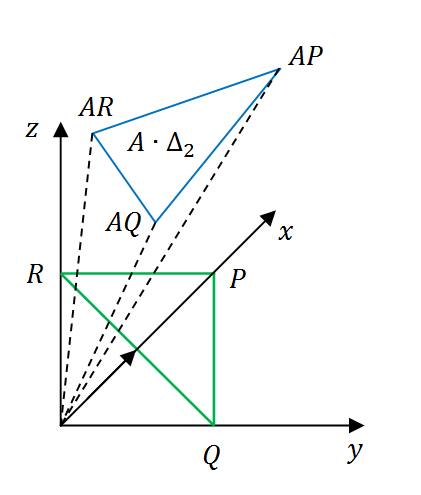
\includegraphics[scale=0.8]{l15_3.png}\\
\end{center}
Функция $c(x, y)=\cfrac{\rho(\varphi(x), \varphi(y))}{\rho(x, y)}$ непрерывна на компактном $\Delta$, причем $c(x, y)<1$. Тогда существует $\varepsilon:~\forall x, y~~c(x, y)<\varepsilon<1$, значит $\varphi$ --- сжимающее отображение (оно сжимает расстояние в $\geqslant \varepsilon$ раз).\\
Воспользуемся теоремой о сжимающем отображении. Здесь $\hat \lambda>0$ (так как $\bar x\in \Delta$, то $\bar x\neq \bar 0$, так что $Ax>0$, $|Ax|_1$ равен сумме всех координат вектора $A\bar x$, а значит >0).\\
$$x=\cfrac{1}{\lambda}Ax>\bar 0$$
Это единственный положительный собственный вектор (как неподвижная точка).
\end{proof}
\begin{center}
    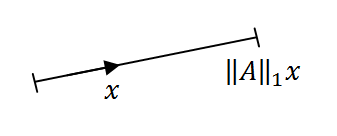
\includegraphics[scale=0.8]{l15_4.png}\\
\end{center}
$$||A||_1=\underset{|x|_1=1}{max}\cfrac{|Ax|_1}{|x|_1} \geqslant \rho(A)$$
\[\bar x \rightsquigarrow |\bar x|= \begin{pmatrix}
|x_1|\\
\vdots\\
|x_n|\\
\end{pmatrix}\]
Тогда $|\bar x|_1=||\bar x||_1,~|Ax|_1\leqslant |A|\bar x||_1.$ Значит $\underset{|x|=1}{max}|Ax|_1=\underset{\bar x \in \Delta}{max}|Ax|_1=||A||_1>\rho(A)$. Оценка $||A||_1 \geqslant \hat \lambda$.
\begin{theorem}[Перрона-Фробениуса]
    Если $A\geqslant 0$ --- неразложимая матрица, то 
\begin{enumerate}
    \item $\exists \hat \lambda_A \geqslant 0$, причем $\hat \lambda_A=\rho(A)$ --- самое большое по модулю собственное значение $A$
    \item при этом соответствующий собственный вектор $\hat x_A \geqslant 0$
    \item если при этом $A\bar y \geqslant \mu \bar y$ для некоторого $\bar y \geqslant \bar 0,~\mu \in \mathbb{R}$, то $\mu \leqslant \hat \lambda_A$
    \item в частности, для любого собственного значения $\lambda$ матрицы $A$ всегда $|\lambda|\leqslant \hat \lambda_A$
\end{enumerate}
\end{theorem}
\begin{proof}
    Пусть $\forall \bar x \geqslant \bar 0~~r_x=\underset{x_i \neq 0}{min} \cfrac{(Ax)_i}{x_i}=max \{ \rho >0 ~~|~~\rho x \leqslant Ax \},~~\rho \leqslant \cfrac{(Ax)_i}{x_i}$.\\
Тогда пусть $M=S_1 \cap \mathbb{R}^n_{\geqslant 0} = \{ x_1 \geqslant 0, \cdots, x_n \geqslant 0~~|~~x_1^2+\cdots +x_n^2=1\}$, где $S_1$ радиуса один.\\
Найдем $\underset{x}{max}~r_x$. Почему он существует?
\begin{enumerate}
    \item $r_x$ непрерывна по $\bar x$ при $\bar x \in \mathbb{R}^n_{>0}$ (то есть $\bar x >0$).\\
    Но если $y=\cfrac{x}{|x|}$, то $y \in M$ и $r_x=r_y$, поэтому $$\underset{x \geqslant \bar 0}{max}~r_x=\underset{\bar x \in M}{max}~r_y$$
    До этого было утверждение о том, что если матрица $A$ --- неразложима, \\то $B=(E+A)^{n-1}>0$. Пусть $N=B(M)= \{\bar z =(E+A)^{n-1} y~~|~~y \in M \}$, тогда $N \subset \mathbb{R}^n>0$.\\
    Если $y\in M$, то $r_y y \leqslant Ay$ и для $z=By$ $$r_yB_y \leqslant AB_y$$ (То есть $AB=BA$). Значит $r_y z \leqslant Az$ $$r_y \leqslant \cfrac{|Az|_i}{|z|_i},~~\forall i=1,\cdots, n$$ $$r_y \leqslant r_z$$
    Так как $$\underset{x \geqslant 0}{max}~r_x=\underset{y \in M}{max}~r_y \leqslant \underset{z\in B}{max}~r_z \leqslant \underset{x\geqslant 0}{max} ~r_x,$$ значит существует $$\underset{z\in N}{max}~r_z=\underset{x \geqslant 0}{max} ~r_x = \underset{y\in M}{max} ~r_y$$
    (так как $N$ --- компактно, $r$ непрерывно на $N \subset \mathbb{R}^n>0$)\\
    Обозначим $r=\hat \lambda =\underset{z\in N}{max}~r_z$. Так как $u=(1 \cdots 1)^T>0$, то $r_u-\underset{i}{min}\cfrac{|A_i|_1}{1}>0$ (так как $A$ разложима), то $r>0$.
    \item Докажем, что $r$ --- собственное значение, то есть найдем собственный вектор. Пусть $$r=r_z,~z=(E+A)^{n-1}y,~(E+A)^{n-1} \in N,~y\in M$$
    Докажем, что $Az=rz$, то есть $\bar z>0$ --- собственный вектор с собственным значением $\hat \lambda=r>0$. Сначала докажем $A\bar y=r \bar y$. Иначе $Ay-ry \geqslant 0,~B(Ay-ry)>0$ $$ABy-rBy=Az-rz>0$$ $$Az>rz \Rightarrow Az> \varepsilon rz, ~\varepsilon >1$$
    Тогда $\varepsilon r \leqslant \cfrac{Az_i}{z_i}$ для всех $i$. $\varepsilon r \leqslant r$ --- противоречие с $\varepsilon >1$. Тогда $y$ --- собственный вектор $$Ay=ry.$$ Но тогда и $z$ --- собственный вектор, так как $$BAy=rBy$$ $$ABy=rBy$$ $$Az=rz$$
    $z>0$ --- собственный вектор с собственным значением $\hat \lambda =r>0$.
    $$(z=(A+E)^{n-1}y=(1+\hat \lambda)^{n-1} \bar y>0 \Rightarrow \bar y>0)$$
    \item Надо доказать, что если $A\bar t \geqslant \mu \bar t$ для некоторого $\bar t \geqslant \bar 0$, то $\mu \leqslant \hat \lambda$. Можем считать $t \in M$, тогда $$At \geqslant \mu t \Rightarrow \mu \leqslant \cfrac{(At)_i}{t_i}$$ то есть $At \geqslant \mu t \Leftrightarrow \mu \leqslant r_t \leqslant \underset{t\in M}{max}~r_t=r=\hat \lambda$.
    \item Надо доказать, что если $\lambda$ --- другое собственное значение, то $|\lambda|\leqslant \hat \lambda$. Пусть $A\bar x=\lambda \bar s$, где $s\neq 0$ --- собственный вектор. Можем считать, что $|s|_2=1$. При этом если 
    \[|\bar s| = \begin{pmatrix}
    |s_1|\\
    \vdots\\
    |s_n|\\
    \end{pmatrix}\]
    (модуль $\bar s$), то $$A|\bar s| \underset{A\geqslant 0}{\geqslant} |\bar{As}|=|\lambda||\bar s|$$
    Так как $|\bar s| \geqslant 0$ (из 3.), то $|\lambda|\leqslant \hat \lambda$. В частности, $\hat \lambda=\rho(A)$
    $$\hat \lambda =\underset{\underset{x\in \Delta}{\underset{x\in M,}{\bar x>0,}}}{max} \underset{i:x_i\neq 0}{~min}\cfrac{(Ax)_i}{x_i}$$
\end{enumerate} 
\end{proof}
\textbf{Пример 1.}
Найти ранги.
\begin{center}
    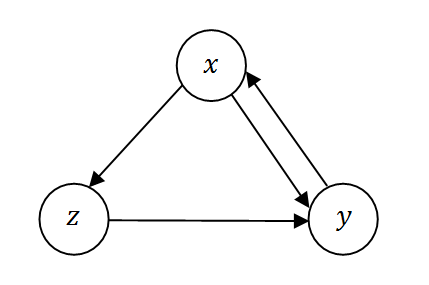
\includegraphics[scale=0.8]{l15_5.png}\\
\end{center}
\[P = \begin{pmatrix}[r]
0 & \cfrac{1}{2} & \cfrac{1}{2}\\
1 & 0 & 0\\
0 & 1 & 0\\
\end{pmatrix}\]
$$(x, y, z)P=(x, y, z)$$
Получим (0.4, 0.4, 0.2).
\subsection{Метод вращений (метод Якоби)}
Пусть матрица $A$ --- симметрическая (матрица $A^*A$ --- всегда симметрическая). Хотим построить процесс $$A_0=A_1,\cdots, A_k \to \Lambda$$
$$T_0=E, T_1, \cdots, T_k \to T$$
$$A=T\Lambda T^{-1}=T \Lambda T^T,$$
$\Lambda$ --- диагональная матрица.\\
Последовательные матрицы перехода $$A_{k+1}=T_{ij}^TA_kT_{ij},$$
$T_{ij}$ --- матрица простых вращений.
$$T_{k+1}=T_kT_{ij}$$
В матрице $A_k$ находим элемент, лежащий не на диагонали, с максимальным модулем $a_{ij}^{(k)}$.
\[ 
T_{ij}=
\left(
\begin{BMAT}[8pt]{ccccccccccc}{ccccccccccc}
1 &   &  & \vdots & & & & \vdots & & &   \\
& \ddots &  & \vdots & & O & & \vdots & & O &    \\
&  & 1 & \vdots & & & & \vdots & & & \\
\cdots & \cdots & \cdots & cos~\varphi & \cdots & \cdots & \cdots & -sin~\varphi & \cdots & \cdots & \cdots\\
& & & \vdots & 1 & & & \vdots & & &  \\
& O & & \vdots &  & \ddots & & \vdots & & O &   \\
& & & \vdots &  & & 1 & \vdots & & & \\
\cdots & \cdots & \cdots & sin~\varphi & \cdots & \cdots & \cdots & cos~\varphi & \cdots & \cdots & \cdots\\
& & & \vdots & &  & & \vdots & 1 & & \\
& O & & \vdots & & O & & \vdots & & \ddots &  \\
& & & \vdots & &  & & \vdots & & & 1 \\
\end{BMAT} 
\right),
\]
где $cos~\varphi$ и $-sin~\varphi$ стоят в $i$ строке, а $sin~\varphi$ и $cos~\varphi$ в $j$ строке.\\
Угол выбираем так, чтобы $$a_{ij}^{(k+1)}=(cos^2 \varphi-sin^2 \varphi)a_{ij}^{(k)}+cos \varphi \cdot sin \varphi (a_{ij}^{(k)}-a_{ii}^{(k)})$$
$$a_{ij}^{(k+1)}=0$$
$$tg ~2\varphi =\cfrac{2a_{ij}^{(k)}}{a_{ii}^{(k)}-a_{jj}^{(k)}},~~|\varphi|\leqslant \cfrac{\pi}{4}$$
$$cos ~2\varphi=\cfrac{1}{\sqrt{1+tg^2 ~2\varphi}}$$
$$cos ~\varphi =\sqrt{\cfrac{1+cos ~2\varphi}{2}}$$
$$sin ~\varphi =\pm \sqrt{\cfrac{1-cos ~2\varphi}{2}}$$
Знак $sin \varphi$ равен знаку $a_{ij}^{(k)}(a_{ii}^{(k)}-a_{jj}^{(k)})$.\\
\\
\textbf{Пример 2.}\\
Найти собственные значения матрицы $A$ методом вращений.\\
\[A = \begin{pmatrix}[r]
17 & -2 & -2\\
-2 & 14 & -4\\
-2 & -4 & 14\\
\end{pmatrix}\]
\[T_{23} = \begin{pmatrix}
1 & 0 & 0\\
0 & cos ~\varphi & -sin ~\varphi\\
0 & sin ~\varphi & cos ~\varphi\\
\end{pmatrix}\]
$$tg ~2\varphi =\cfrac{2 a_{23}}{a_{22}-a_{33}}=\cfrac{2\cdot (-4)}{14-14}=-\infty$$
$$2\varphi =-\cfrac{\pi}{2},~~\varphi=-\cfrac{\pi}{4}$$
Подставим значения в матрицу $T_{23}$.
\[T_{23} = \begin{pmatrix}
1 & 0 & 0\\
0 & \cfrac{\sqrt{2}}{2} & \cfrac{\sqrt{2}}{2}\\
0 & -\cfrac{\sqrt{2}}{2} & \cfrac{\sqrt{2}}{2}\\
\end{pmatrix}\]
\[A_1=A_{k+1} = T_{23}^T A T_{23}=\begin{pmatrix}[r]
1 & 0 & 0\\
0 & \cfrac{\sqrt{2}}{2} & -\cfrac{\sqrt{2}}{2}\\
0 & \cfrac{\sqrt{2}}{2} & \cfrac{\sqrt{2}}{2}\\
\end{pmatrix} \begin{pmatrix}[r]
17 & -2 & -2\\
-2 & 14 & -4\\
-2 & -4 & 14\\
\end{pmatrix} \begin{pmatrix}[r]
1 & 0 & 0\\
0 & \cfrac{\sqrt{2}}{2} & \cfrac{\sqrt{2}}{2}\\
0 & -\cfrac{\sqrt{2}}{2} & \cfrac{\sqrt{2}}{2}\\
\end{pmatrix}=\begin{pmatrix}
17 & 0 & -\cfrac{4}{\sqrt{2}}\\
0 & 18 & 0\\
-\cfrac{4}{\sqrt{2}} & 0 & 10\\
\end{pmatrix}\]
\[T_{13} = \begin{pmatrix}
cos ~\varphi & 0 & -sin ~\varphi\\
0 & 1 & 0\\
sin ~\varphi & 0 & cos ~\varphi\\
\end{pmatrix}\]
$$tg ~2\varphi=\cfrac{2\cdot (-\cfrac{4}{\sqrt{2}})}{17-10}=-\cfrac{8}{7\sqrt{2}}$$
$$cos ~2\varphi=\cfrac{1}{\sqrt{1+\cfrac{64}{49\cdot 2}}}=\cfrac{7}{9}$$
$$cos ~\varphi=\sqrt{\cfrac{1+\cfrac{7}{9}}{2}}=\cfrac{2\sqrt{2}}{3}$$
$$sin ~\varphi=-\sqrt{\cfrac{1-\cfrac{7}{9}}{2}}=-\cfrac{1}{3}$$
Подставим значения в матрицу $T_{13}$.
\[T_{13} = \begin{pmatrix}
\cfrac{2\sqrt{2}}{3} & 0 & \cfrac{1}{3}\\
0 & 1 & 0\\
-\cfrac{1}{3} & 0 & \cfrac{2\sqrt{2}}{3}\\
\end{pmatrix}\]
\[A_2= T_{13}^T A_1 T_{13}=\begin{pmatrix}
\cfrac{2\sqrt{2}}{3} & 0 & -\cfrac{1}{3}\\
0 & 1 & 0\\
\cfrac{1}{3} & 0 & \cfrac{2\sqrt{2}}{3}\\
\end{pmatrix} \begin{pmatrix}
17 & 0 & -\cfrac{4}{\sqrt{2}}\\
0 & 18 & 0\\
-\cfrac{4}{\sqrt{2}} & 0 & 10\\
\end{pmatrix} \begin{pmatrix}
\cfrac{2\sqrt{2}}{3} & 0 & \cfrac{1}{3}\\
0 & 1 & 0\\
-\cfrac{1}{3} & 0 & \cfrac{2\sqrt{2}}{3}\\
\end{pmatrix}=\begin{pmatrix}
18 & 0 & 0\\
0 & 18 & 0\\
0 & 0 & 9\\
\end{pmatrix}\]
Получили собственные значения $\lambda_1=\lambda_2=18,~\lambda_3=9$.\\
Найдем соответствующие собственные векторы.
$$T_1=T_0T_{23}=ET_{23},~T_2=T_1T_{13}$$
\[T_2 = \begin{pmatrix}[r]
\cfrac{4}{3\sqrt{2}} & 0 & \cfrac{1}{3}\\
-\cfrac{1}{3\sqrt{2}} & \cfrac{\sqrt{2}}{2} & \cfrac{2}{3}\\
-\cfrac{1}{3\sqrt{2}} & \cfrac{\sqrt{2}}{2} & \cfrac{2}{3}\\
\end{pmatrix}\]
Каждый из столбцов матрицы $T_2$ является собственным вектором $\lambda_1,~\lambda_2$ и $\lambda_3$ соответственно.
\subsection{Домашнее задание 15}\begin{enumerate}
    \item Найти собственные векторы и собственные значения методом вращений (методом Якоби).
    \begin{enumerate}
        \item \[\begin{pmatrix}[r]
        2 & 2 & -2\\
        2 & 5 & -4\\
        -2 & -4 & 5\\
        \end{pmatrix}\]
        \item \[\begin{pmatrix}[r]
        6 & -2 & 2\\
        -2 & 5 & 0\\
        2 & 0 & 7\\
        \end{pmatrix}\]
        \item \[\begin{pmatrix}
        3 & 2-i & 0\\
        2+i & 7 & 0\\
        0 & 0 & 3\\
        \end{pmatrix},\] матрица удовлетворяет условию $A^*=A$, что гарантирует, что у нее есть диагональная форма.
    \end{enumerate}
\end{enumerate}